\documentclass[14pt,a4paper]{extarticle}
\usepackage[T2A]{fontenc}
\usepackage[utf8]{inputenc}
\usepackage[english,russian]{babel}
\usepackage{lmodern}
\usepackage{geometry}
\usepackage{array}
\usepackage{tabularx}
\usepackage{longtable}
\usepackage{ltablex}
\usepackage{booktabs}
\usepackage{hyperref}
\usepackage{indentfirst}
\usepackage{microtype}
\usepackage{graphicx}
\usepackage{setspace}
\usepackage{listings}
\usepackage{graphicx}
\usepackage{caption}
\usepackage{float}
\usepackage{tocloft}
\usepackage{titlesec}
\usepackage{newtxtext,newtxmath}

\titleformat{\section}        % форматируем \section
  {\normalfont\bfseries}      % стиль: обычный + жирный
  {\thesection.}              % номер секции с точкой
  {2mm}                       % расстояние между номером и текстом
  {}                           % перед заголовком можно добавить что-то
\titlespacing*{\section}{1.5cm}{*3}{*1}  % {отступ слева}{отступ сверху}{отступ снизу}

\captionsetup{justification=centering}
\renewcommand{\ttdefault}{cmtt}
\keepXColumns
\setlength{\parindent}{3em}
\newgeometry{left=2.5cm,right=2.5cm,top=3cm,bottom=2.5cm}

\renewcommand{\contentsname}{\hspace*{4em}{\smallСодержание}}
\setlength{\cftbeforesecskip}{0.5em}
\renewcommand{\cftsecleader}{\cftdotfill{\cftdotsep}}
\renewcommand{\cftsecaftersnum}{.\hspace{2mm}}

\title{Отчёт по "Корпоративные информационные системы"}
\author{Выполнил студент группы М-РИТ-25-1, Станиславчук Сергей}

\begin{document}

\setstretch{1.5}
\noindent
\begin{minipage}[t]{0.01\textwidth}
    \includegraphics{~/programmer/++Programmer/5_1/LSTU.jpg}
\end{minipage}%
\begin{minipage}[c]{1.1\linewidth}
    \centering
    {\small
    МИНИСТЕРСТВО НАУКИ И ВЫСШЕГО ОБРАЗОВАНИЯ РФ \\[1em]
    ФЕДЕРАЛЬНОЕ ГОСУДАРСТВЕННОЕ БЮДЖЕТНОЕ \\
    ОБРАЗОВАТЕЛЬНОЕ УЧРЕЖДЕНИЕ ВЫСШЕГО ОБРАЗОВАНИЯ \\
    «ЛИПЕЦКИЙ ГОСУДАРСТВЕННЫЙ ТЕХНИЧЕСКИЙ УНИВЕРСИТЕТ»
    }
\end{minipage}%

\vspace{3em}

\noindent
\hspace{1em}%
\begin{minipage}[t]{0.8\textwidth}
\textbf{Институт} \hspace{2em} компьютерных наук \\
\textbf{Кафедра} \hspace{2em} автоматизированных систем управления
\end{minipage}


\vspace{6em}

\begin{center}
\textbf{Практическая работа №1} \\
по дисциплине \\ <<Корпоративные информационные системы>>
\end{center}

\vspace{6em}

\noindent
\begin{tabular*}{\textwidth}{@{\extracolsep{\fill}} l c r }
    Студент М-РИТ-25-1 & \makebox[4cm]{\hrulefill} & Станиславчук С.М. \\[2em]
Руководитель & \\
К.т.н., доцент & \makebox[4cm]{\hrulefill} & Галкин А.В. \\
\end{tabular*}

\vfill
\begin{center}
    Липецк, 2026
\end{center}

\thispagestyle{empty}

\newpage
\tableofcontents
\newpage

\section{Характеристика предметной области}

Выбранная АИС: “Система управления учебным процессом в высшем
учебном заведении” (Личный кабинет).

Система разработана с учетом трех типов пользователей: студент,
преподаватель и администратор.

Процесс работы происходит следующим образом: администратор системы
(superuser) до начала учебного семестра генерирует расписание предметов на
семестр; преподаватель просматривает расписание предметов, выставляет
оценки студентам, также может предоставить отчет успеваемости студентов,
у которых он ведет занятия; студент также имеет доступ к просмотру
расписания предметов своей группы, а также может просматривать
полученные оценки. Таким образом, система позволяет контролировать
учебный процесс с обеих сторон – и для студента, и для преподавателя.

\section{Описание бизнес-процесса}

\textbf{Границы моделируемого процесса:} процесс начинается с ввода преподавателем оценки за результат обучения студента и заканчивается предоставлением актуальной информации об успеваемости.

\textbf{Входные потоки:} данные о студенте, учебной группе, дисциплине и преподавателе, оценка.

\textbf{Выходные потоки:} сохранённая оценка, средний балл по дисциплине, отчёты об успеваемости.

\textbf{Показатели процесса:} количество и значения полученных оценок, средний балл студента по дисциплине за семестр, результаты успеваемости за выбранный период.

\textbf{Персонал:} преподаватели, студенты, администраторы образовательного процесса.

\textbf{Исполнители отдельных функций:} преподаватель вводит и редактирует оценки; информационная система проверяет и сохраняет данные, рассчитывает средний балл и формирует отчёты; студент просматривает свою успеваемость; администратор анализирует успеваемость студентов.

\section{Модель бизнес-процесса}

Модель бизнес-процесса “Учет успеваемости и оценок” в нотации BPMN
представлена на рисунке 1.

\begin{figure}[H]
    \label{fig:pic1}
    \centering
    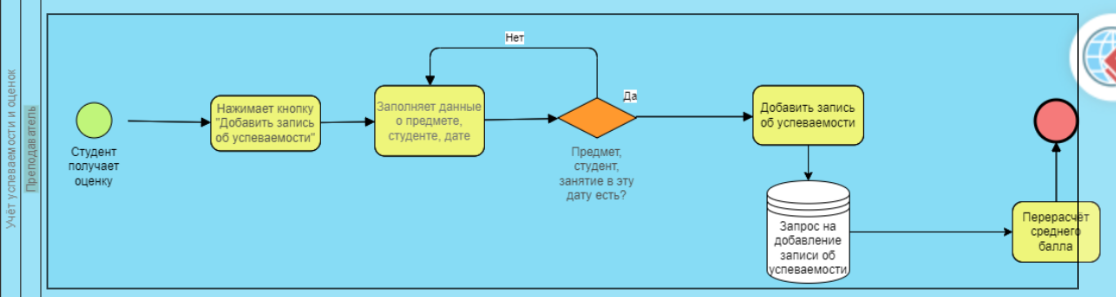
\includegraphics[width=0.78\textwidth]{pic1.png}
    \refstepcounter{figure}
    \caption*{Рисунок \thefigure\ — BPMN модель “Учет успеваемости и оценок”}
\end{figure}

\end{document}
